\documentclass[tikz]{standalone}
\usepackage{amsmath}
\usepackage{pgf}
\usepackage{pgfplots}
\pgfplotsset{compat=1.18,}
% \listfiles
\begin{document}
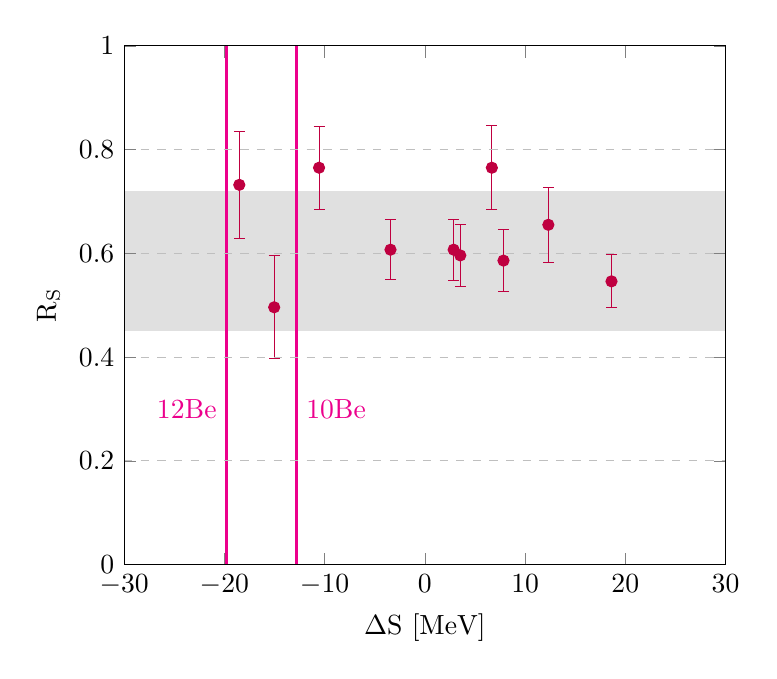
\begin{tikzpicture}
	\begin{axis}[
		width=0.63\linewidth,
		scale only axis,
		xlabel={$\Delta$S [MeV]},
		ylabel={$\text{R}_{\text{S}}$},
		xmin=-30, xmax=30,
		ymin=0, ymax=1,
		ymajorgrids=true, yminorgrids=true,
		grid style = {dashed},
		axis on top,
		]
		\addplot[fill=black!12, draw=none, forget plot] coordinates {(\pgfkeysvalueof{/pgfplots/xmin}, 0.45) (\pgfkeysvalueof{/pgfplots/xmax}, 0.45)  (\pgfkeysvalueof{/pgfplots/xmax}, 0.72) (\pgfkeysvalueof{/pgfplots/xmin}, 0.72)};
		\addplot [purple, only marks,
			error bars/.cd,
			y dir=both, y explicit,
		] table [y error=u] {
				x		   y      u
				-18.508    0.732  0.103
				-15.028    0.496  0.099
				-10.552    0.765  0.080
				-3.425    0.607  0.058
				2.873    0.607  0.059
				3.536    0.596  0.060
				6.685    0.765  0.081
				7.845    0.586  0.060
				12.320    0.655  0.072
				18.619    0.546  0.051
			};
		\draw[magenta, very thick] (axis cs:-12.8,\pgfkeysvalueof{/pgfplots/ymin}) -- (axis cs:-12.8,\pgfkeysvalueof{/pgfplots/ymax});
		\node[magenta, right] at (-12.8, 0.3) {10Be};
		\draw[magenta, very thick] (axis cs:-19.8,\pgfkeysvalueof{/pgfplots/ymin}) -- (axis cs:-19.8,\pgfkeysvalueof{/pgfplots/ymax});
		\node[magenta, left] at (-19.8, 0.3) {12Be};
	\end{axis}
\end{tikzpicture}
\end{document}